\documentclass[a4paper, 10pt]{article}%тип документа

%Русский язык
\usepackage[T2A]{fontenc} %кодировка
\usepackage[utf8]{inputenc} %кодировка исходного кода
\usepackage[english,russian]{babel} %локализация и переносы

\usepackage{multirow}

%Вставка картинок
\usepackage{cellspace, graphicx, makecell}
\DeclareGraphicsExtensions{.pdf,.png,.jpg}

\renewcommand\cellspacetoplimit{3pt}
\renewcommand\cellspacebottomlimit{3pt}
\newcommand\rowincludegraphics[2][]{\raisebox{-0.45\height}{\includegraphics[#1]{#2}}}

%Производные
\usepackage{physics}

%Математика
\usepackage{amsmath, amsfonts, amssymb, amsthm, mathtools}
\usepackage[left=10mm, top=20mm, right=18mm, bottom=15mm, footskip=10mm]{geometry}

%Заголовок
\author{Дербенев Никита Максимович}
\title{Лабораторная работа 1.4.8\\
	Измерение модуля Юнга методом аккустического резонанса}
\date{26 октября 2023}
\begin{document}
	\maketitle
	\paragraph {Цель работы:}
		Исследовать явление акустического резонанса в тонком стержне; измерить скорость распространения продольных звуковых колебаний в тонких стержнях из различных материалов и различных размеров; измерить модули Юнга различных материалов.
	\paragraph{В работе используются:}
	\begin{enumerate}
		\item Генератор звуковых частот
		\item Частотомер
		\item Осциллограф
		\item Электромагнитные излучатель и приёмник колебаний
		\item Набор стержней из различных материалов
	\end{enumerate}
	\paragraph{Ход работы:}
	\begin{enumerate}
		\item Настроим частотометр и осциллограф для работы с установкой
		\item Поместим медный стержень на подставку, придвинем максимально близко к торцам датчики, не допуская соприкосновения со стержнем. Расстояние между торцами стержня и датчиками получилось < 0.5мм.
		\item Определим приблизительную частоту первого резонанса медного стержня по формуле:
		\[f_1 = \dfrac{u}{2L} \approx \dfrac{3.7 \cdot 10^3}{2 \cdot 0.6} \approx 3.083 \text{ кГц}\]
		\item Плавно изменяя частоту генератора в районе 3 кГц, найдем положение резонанса, при котором амплитуда сигнала будет максимальна и изображение на осциллографе будет представлять собой бочку (на самом деле это обрезанный эллипс, ибо датчик жестко обрезает выходной сигнал). Запишем значение резонансной частоты в табл. 1.
		\item Получим резонансы на частотах, соответствующих кратным гармоникам. Для этого, плавно перестраивая генератор, добемсяь резонанса вблизи частот $f_n = nf_1$, где $n = 2, 3, ...$ Запишем измеренные значения частот в табл. 1.
		\begin{table}[h]
			\centering
			\caption{Значения резонансых частот}
			\begin{tabular}{|l||c|c|c|c|c|c|c|c|c|c|c|}
				\hline
				№ гармоники & 1 & 2 & 3 & 4 & 5 & 6 & 7 & 8 & 9 & 10 & 11 \\
				\hline
				Медь   & 3.2489 & 6.4596 &  9.7282 & 12.9987 & 16.2359 & 19.4556 & 22.6828 & 25.9312 & 29.1485 & 32.4021 & 35.6396 \\
				\hline
				Дюраль & 4.2274 & 8.4898 & 12.7445 & 16.9726 & 21.1814 & 25.3987 & 29.5944 & 33.8376 & 38.0211 & 42.3422  & - \\
				\hline
				Сталь  & 4.1291 & 8.2701 & 12.3921 & 16.5571 & 20.6358 & 24.7582 & 28.8421 & - & - & - & - \\
				\hline
			\end{tabular}
		\end{table}
		\item Повторим пункты 2-5 для дюрали и стали.
		\item Определим плотность материалов стержней. Для этого взвесим и измерим штангенциркулем линейные размеры небольшого образца цилиндрической формы, изготовленного из исследуемого материала. Результаты запишем в табл. 2:
		\[\rho = \dfrac{4m}{\pi l d^2}\]
		\[\varepsilon_\rho = \varepsilon_m + \varepsilon_\pi + \varepsilon_l + 2\varepsilon_d \approx 2\varepsilon_d\]
		\[\sigma_\rho = \varepsilon_\rho\rho\]
		\item Построим график зависимостей резонансной частоты от номера гармоники (рис. 1). Видим, что точки хорошо ложаться на прямые $f_n = kn$. Вычислим скорость распространения волн в стержне по МНК и запишем в табл. 3:
		\[u = 2kL\]
		\[\varepsilon_u = \varepsilon_L + \varepsilon_k \approx \varepsilon_k = \dfrac{\sigma_k}{k}\]
		\[\sigma_u = u\varepsilon_u\]
		\item Определим модули Юнга различных материалов и запишем в табл. 3:
		\[E = u^2\rho\]
		\[\varepsilon_E = 2\varepsilon_u + \varepsilon_rho\]
		\[\sigma_E = \varepsilon_EE\]
		\begin{table}
			\centering
			\caption{Параметры кусочков стержней}
			\begin{tabular}{|c|c|c|c|}
				\hline
				Материал & Медь & Дюраль & Сталь \\
				\hline
				$m$, г & 39.366 & 37.072 & 26.017 \\
				\hline
				$d$, мм & 11.9 & 12.2 & 12.1 \\
				\hline
				$l$, мм & 39.6 & 41.1 & 29.5 \\
				\hline
				$S, \text{ мм}^2$ & 111.22 & 116.90 & 114.99 \\
				\hline
				$V, \text{ мм}^3$ & 4404.3 & 4804.6 & 3392.2 \\
				\hline
				$\rho, \frac{\text{кг}}{\text{м}^3}$ & $8930 \pm 300$ (3.4\%)  & $7720 \pm 250$ (3.3\%) & $7670 \pm 250$ (3.3\%) \\
				\hline
			\end{tabular}
		\end{table}
		\begin{table}
			\centering
			\caption{Параметры стержней}
			\begin{tabular}{|c|c|c|c|}
				\hline
				Материал & Медь & Дюраль & Сталь \\
				\hline
				$f_1$, кГц & $3.2391 \pm 0.0016$ (0.05\%) & $4.2261 \pm 0.0032$ (0.08\%) & $4.1197 \pm 0.0042$ (0.10\%) \\
				\hline
				$u, \frac{\text{м}}{c}$ & $3887 \pm 2$ (0.05\%) & $5071 \pm 4$ (0.08\%) & $4994 \pm 5$ (0.10\%) \\
				\hline
				$E$, ГПа & $135 \pm 5$ (3.5\%) & $199 \pm  7$ (3.5\%) & $191 \pm 7$ (3.5\%) \\
				\hline
			\end{tabular}
		\end{table}
		\begin{figure}
			\centering
			\caption{График зависимости частоты от номера гармоники ($f_n(n)$)}
			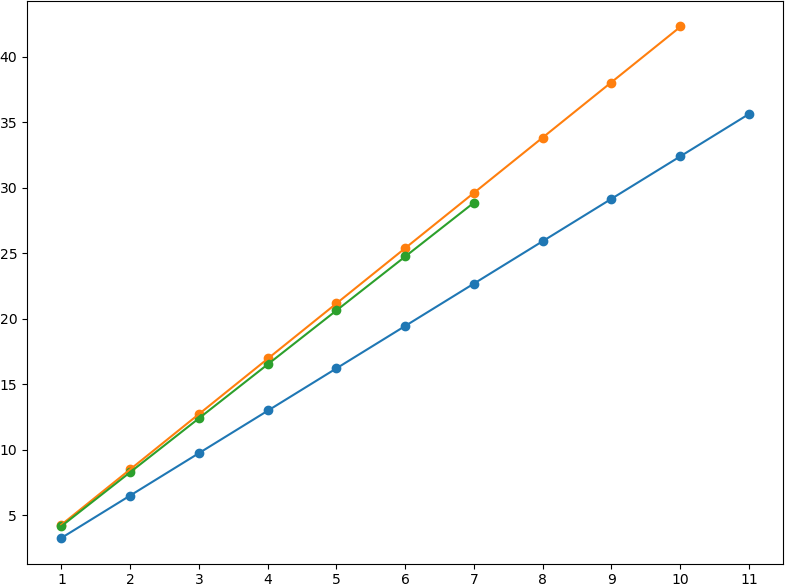
\includegraphics{Figure_1}
		\end{figure}
		\item Добьемся возникновения резонанса в стержне из дюрали на частоте $f_1/2$. Добьемся возникновения на экране осциллографа фигуры Лиссажу (рис. 2).
		\begin{figure}
			\centering
			\caption{Резонанс на $f_1/2$}
			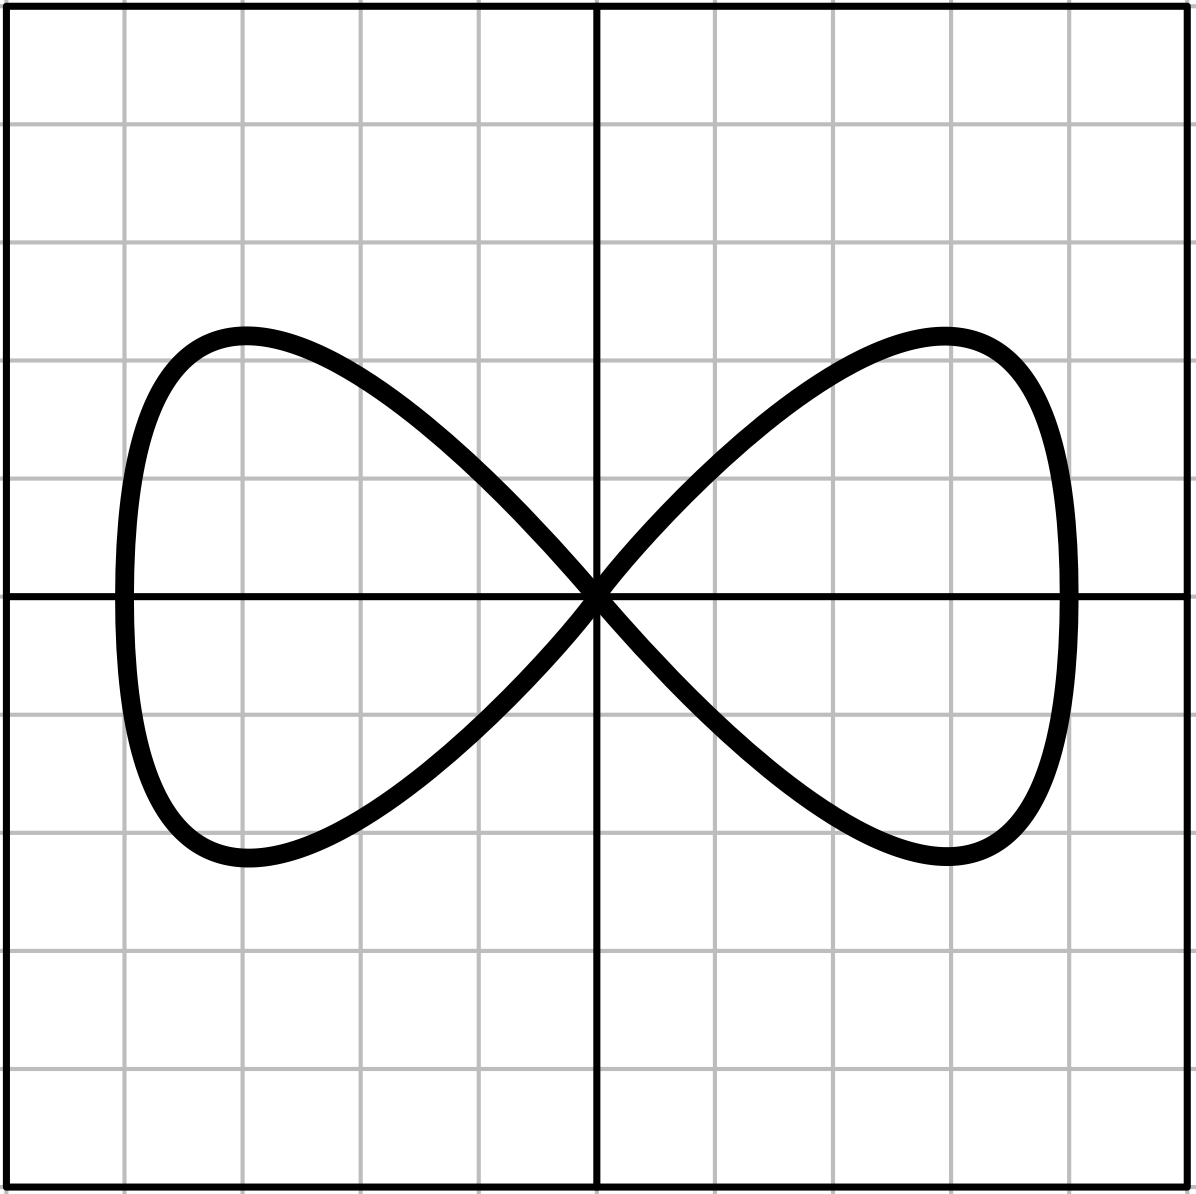
\includegraphics{lis}
		\end{figure}
		\item Измерим добротность колебаний в дюралюминиевом стержне. Для этого определим частоты вблизи резонанса, при которых амплитуда сигнала достигает $\dfrac{U_{max}}{\sqrt{2}}$:
		\[f_1 = 4238.0 \text{ Гц}\]
		\[f_2 = 4230.1\text{ Гц}\]
		\[\Delta_f = \dfrac{f_1+f_2}{2} \approx 4.0 \text{ Гц}\]
		\[U = \dfrac{f_n}{\Delta_f} \approx 1058\]
	\end{enumerate}
	\paragraph {Вывод:}
		Метод аккустического резонанса - достаточно точный метод определения модуля Юнга материалов с низкой погрешностью (3.5\%). Основная погрешность связана с определением плотности материалов, а точнее с определением диаметра стержней. Ее можно уменьшить, если измерять диаметр стержней микрометром в разных местах.
\end{document}